Let's train a neural network to classify these digits, using 60,000 input/output examples in \texttt{trainData} dataset for supervised learning and evaluate the performance on 10,000 examples in the \texttt{testData} dataset.

\subsection{Choosing the network architecture}
It would be a good idea to use some well-known architecture that was trained on other platforms. This way we can easily compare the performance. Here are the two architectures I will be working with in this chapter
\begin{enumerate}
  \item Single-layer neural network with $784$ inputs and $10$ neurons. All neurons have softmax activation function. The learning rate is constant and set to $0.5$. The network uses Cross-entropy cost function
\end{enumerate}

\begin{table}[h!]
  \centering
  
  \begin{tabularx}{0.75\textwidth}{|H|CC|}
    \hline
                    & Network \#1       & Network \#2 \\
    \hline
    Architecture    & 784, 10           & 784, 500, 10       \\
    Activations     & Softmax           & Logistic, Softmax \\
    Cost            & Cross-entropy     & Cross-entropy \\
    \hline
  \end{tabularx}
  
  \caption{Table to test captions and labels}
  \label{table:architectures}
\end{table}

\begin{table}[h!]
  \centering
  
  \begin{tabularx}{0.75\textwidth}{|H|CC|}
    \hline
                    & Network \#1       & Network \#2 \\
    \hline
    Batch size      & 100               & 100 \\
    Epochs          & 1000              & 500 \\
    Learning rate   & 0.5               & 0.5 \\
    \hline
  \end{tabularx}
  
  \caption{Table to test captions and labels}
  \label{table:training}
\end{table}

The results obtained after training

\begin{table}[h!]
  \centering
  
  \begin{tabularx}{0.75\textwidth}{|H|CC|}
    \hline
                    & Network \#1       & Network \#2 \\
    \hline
    Accuracy        & 92\%              & 88\% \\
    Training time   & 0:00:38:02.85     & 0:00:38:02.85 \\
    Time per epoch  & 0:00:38:02.85     & 0:00:38:02.85 \\
    \hline
  \end{tabularx}
  
  \caption{Table to test captions and labels}
  \label{table:results}
\end{table}

\subsection{Single-layer neural network (784, 10)}

\begin{lstlisting}
neuralNet := MLNeuralNetwork new initialize: #(784 10).
neuralNet outputLayer activationFunction: (MLSoftmax new).
neuralNet costFunction: (MLCrossEntropy new).
neuralNet lerningRate: 0.5.

neuralNet learningAlgorithm: (MLMiniBatchBackpropagation new).
neuralNet batchSize: 100.
\end{lstlisting}

\begin{lstlisting}
neuralNet learn: trainingData epochs: 1000.
\end{lstlisting}

\begin{figure}[H]
  \centering
  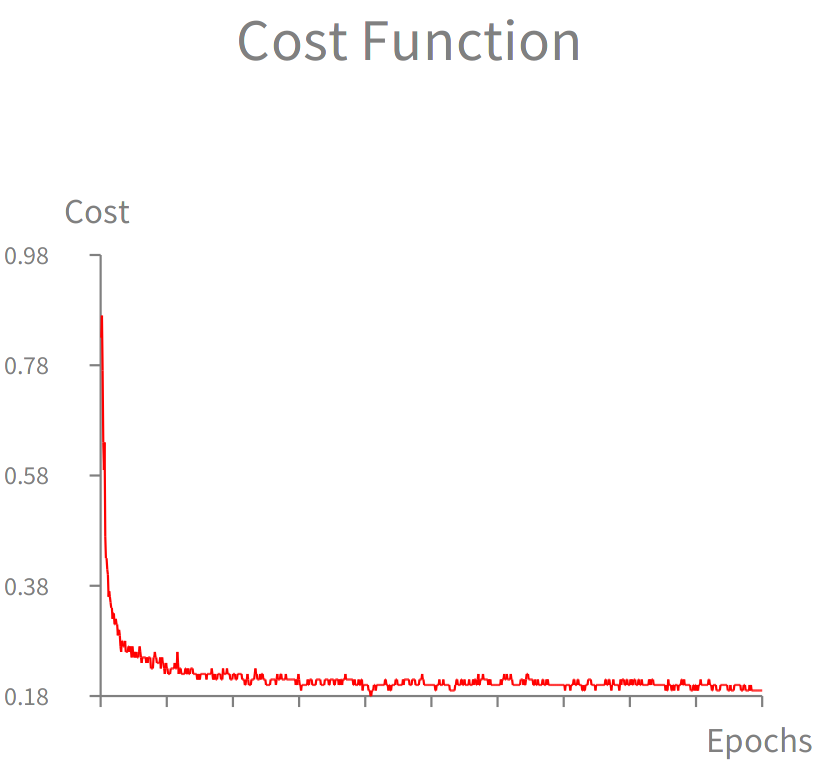
\includegraphics[width=\imgwidth]{cost-784-10}
  \caption{Cost history of a single-layer neural network}
  \label{fig:cost-784-10}
\end{figure}

\subsection{Two-layer neural network (784, 500, 10)}
